\documentclass{article}
% set up the page formatting
\usepackage[a4paper, portrait, margin=2.5cm]{geometry}
\usepackage{multicol}
\usepackage{fancyhdr}
\usepackage{graphicx}
\usepackage{float}

% allow for table of contents to have clickable links
\usepackage{hyperref}

% editable bits
\title{\vspace{-1.5cm}CS261 Group 29 Report}
\author{Ani Bitri, Krister Hughes, Thomas Phuong, Eshan Sharif, Josh Turner, Antoni Zyla}
\date{January 2025}
\fancyfoot[L]{Report}
\fancyfoot[R]{\thepage}

\begin{document}
\maketitle

\section{Preface}

Dorset Software tasked our team with creating a traffic junction simulator. And we fucking did it. 

Dorset Software has tasked our team with the creation of a traffic junction simulator which will be used for the modelling of traffic junctions on various parameters. The system provides data on how these configurations 
affect the traffic flow and the overall efficiency of the junction in comparsion to other configurations. 

This document explains the development process of the system and provide an explanation to the key changes and decisions made throughout the implementation of the prototype. Furthermore,
it will give an insight into the algorithms and formulas used to calculate the traffic flow and efficiency of the junctions.

\section{System Overview}

    \subsection{Purpose}

        Our system is a traffic junction simulator intended to be used by traffic engineers, urban planners and district governments to model and analyse the efficiency of different traffic junction configurations. The
        system includes a frontend interface for users to input their desired configurations, a simulation page to visualise the traffic flow and a results page to display the metrics of the simulation.

    \subsection{Developer Tools Used}

        The sytem was developed using Python and a few of its libraries. This allowd for easier transition between the frontend and backend of the system. The
        fronted was developed using PyQT5 for the GUI and MatPlotLib for aid in the Visualisation of the results. 

        Our team also utilised GitHub for version control and better collaboration between team members.

    \subsection{User Interaction}

        The system is designed to be user-friendly and intuitive. When the application first opens, the user is greeted with the "Input Parameters"
        page where they can input the desired parameters for the simulation.
        
    \subsection{System Architecture and Interaction}

\section{Modifications}

\section{Algorithms and Formulas}

    \subsection{Semaphores}

    \subsection{Traffic Flow}

    \subsection{Calculating Metrics}

    \subsection{Overall Score}

\section{Frontend}

    \subsection{User Interface Design}
    The previous interface design combined the inputs, simulation, and results onto a single screen where you could tab between inputs and parameters. While this worked, 
    a few issues arose when implementing it, such as, cluttered visuals, reduced usability, and a limited possibility of expansion. To address these newly found issues, 
    instead of tabbing between the inputs and parameters pages, we made it so the inputs and parameters, the simulation, and results were given their own unique tab to 
    function on. As a results of implementing the project this way, we found key advantages present in this layout compared to the previous one.

        \subsubsection{Improved Organisation}
        By separating the inputs, simulation, and results into distinct tabs, users can focus on one aspect of the interface at a time. This tabbed approach also enhances 
        the workflow efficiency of the user and gives the user a natural progression to follow between data entry to simulation execution and results analysis.

        \subsubsection{Reduced Clutter}
        The previous design displayed all elements of our user interface on one screen, making it visually overwhelming and difficult to navigate. The new design split of 
        the interface, allowing the user to interact with each section independently, reducing the visual overload and improving the overall ease of use.

        \subsubsection{Increased Space for Additional Features}
        The old layout restricted the ability of add new functionalities due to space constraints as all three segments were on one page. By utilising the tab-based system, 
        we have created for room for additional features such as adding graphs to the results page.

    \subsection{Home Page}

        The user is first greeted with the home page where some general information about the system is displayed. The user can then click the "Go to Input Parameters" button to go to the Inputs Page 
        or click the "Exit" button to exit the application. The image below shows the home page of the system:

        \begin{figure}[H]
            \centering
            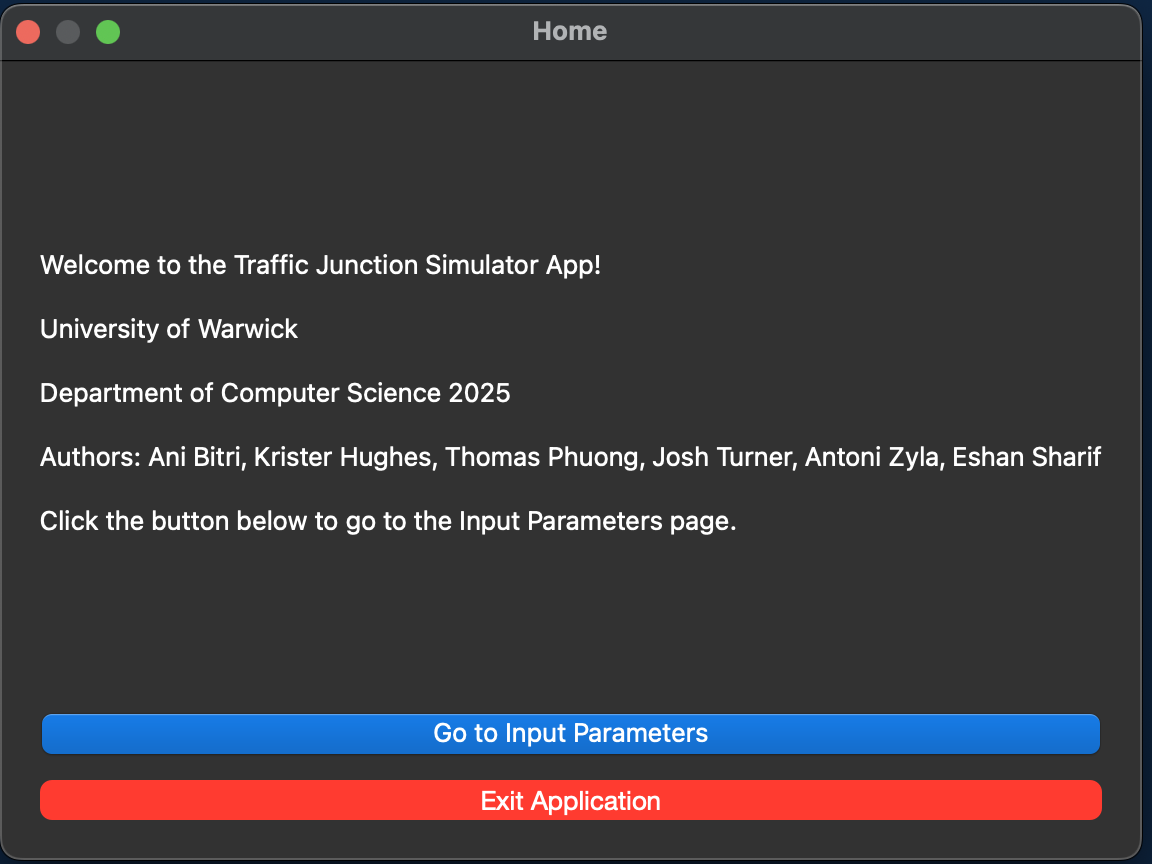
\includegraphics[width=7cm]{img/homepage.png}
            \caption{Home Page of the System}
            \label{fig:homepage}
        \end{figure}
    
    \subsection{Input and Validation Page}

        The Input Page provides a structured interface for configuring traffic flow conditions. The page intially consists of a parent junction box, labelled "Junction 1", which contains child boxes for 
        each direction of traffic flow. Each child box contains input fields for the user to input the desired parameters for the simulation. The image below shows the parent junction box and the child boxes for
        each direction of traffic flow:
        
        \begin{figure}[h!]
            \centering
            \includegraphics[width=\textwidth]{img/inputbox.png}
            \caption{Illustration of the Input Box}
            \label{fig:inputBox}
        \end{figure}

        The parent box also contains two checkboxes for the user to select whether they want to add pedestrian crossing options and whether they want to see the updates on the junction on real time. A visual representation of the
        junction is displayed on the right side of the parent box, which updates in real time as the user inputs the parameters. The image below shows the visual representation:

        \begin{figure}[H]
            \centering
            \includegraphics[width=\textwidth]{img/inputboxextra.png}
            \caption{Illustration of the Input Box with additional options}
            \label{fig:inputBox}
        \end{figure}

        This layout was achieved by using the PyQT library to create the boxes using QGroupBox widgets.

    \subsection{Results Page}

    \subsection{PDF genereation}

    \subsection{Error Handling}
    Within our application, there are many scenarios which require the user to input certain parameters or complete steps in a specific order. The way we handled these problems as a team were by checking and verifying the user's inputs by setting up certain constraints on the input boxes and by displaying error messages with the necessary steps to fix the issue on them.
    \subsubsection{Input Checking}
    On the Input and Parameter page we ensured that the user entered the correct inputs by having certain checks in place:
    \begin{itemize}
        \item When the user enters the VpH exiting each exit, we ensured that the input was an integer, greater or equal to 0, and had an upperbound of 999 VpH.
        \item When the user enters the number of lanes for each exit, the number had to be greater than 0, had an upper bound of 5, and was always an integer.
        \item For the Priority, we made sure that the user could only have a priority that was greater than or equal to 0, at most 4, and was an integer.
        \item If the user had chosen to add a pedestrian crossing, we made sure that the time it takes for people to cross and the number of crossing requests per hour were both greater than 0, less than 1000, and always an integer.
    \end{itemize}
    \subsubsection{Error Messages}
    There are features in our application that require the user to complete steps in a certain order. If the prerequirement is not met for a certain feature, an error message will be displayed:
    \begin{itemize}
        \item If the user chooses to remove an alternate configuration without creating one in the first place, an error message will be displayed that will tell the user too add an alternate configuration before they are able to remove one.
        \item In the scenario that the user decides to generate a report PDF without generating any results, an error message would display: telling the user to press the generate results button in order to generate the results of their configuration before pressing the report button again.
        \item As the user is setting up their junction configuration, if the user does not set a suitable number of lanes, when starting the simulation an error message will display. The error message will prompt the user to change the number of lanes on the exit that has an inconsistent number of lanes and incoming traffic. The error message should tell the user which junction configuration is causing an issue and which direction of traffic flow needs to be changed.
    \end{itemize}

    \subsubsection{Testing}
    In order to check whether our input checking and error messages were prompted at the correct situation, we were required to set up some tests.
    \begin{itemize}
        \item Input Checking
        \begin{itemize}
            \item Boundary Testing
            \begin{itemize}
                \item Tested inputs on both the lower and upper bounds for the valid ranges:
                \begin{itemize}
                    \item For VpH, tested the range 0-999 to ensure values within this range are accepted.
                    \item For the number of lanes, tested the range 1-5 to ensure values within this range are accepted.
                    \item For priority levels, tested the range 0-4 to ensure values within this range are accepted.
                    \item For pedestrian crossing time and number of requests per hour, tested the range 1-999 to ensure values within this range are accepted.
                \end{itemize}
            \end{itemize}
            \item Erroneous Testing
            \begin{itemize}
                \item Tested with non-integer inputs (e.g., strings like "abc" or decimals like 2.5) to ensure only integers are accepted.
                \item Tested with invalid characters (e.g., special characters like "@\#\$") and blank spaces to ensure they are rejected.
                \item Tested values just outside the allowed range (e.g., -1 for VpH, 0 for number of lanes, and 6 for priority) to ensure they are not accepted.
            \end{itemize}
        \end{itemize}
    
        \item Error Messages
        \begin{itemize}
            \item Precondition Testing
            \begin{itemize}
                \item Ensured that error messages were displayed when prerequisites for actions were not met:
                \begin{itemize}
                    \item When attempting to remove an alternate configuration without having created one, an error message is displayed prompting the user to add one first.
                    \item When attempting to generate a report PDF without first generating results, an error message is displayed informing the user to generate results before generating a report.
                    \item when Attempting to start the simulation when the lanes arent balanced with the traffic, the error message should always be raised.
                \end{itemize}
            \end{itemize}
            \item Sequence Testing
            \begin{itemize}
                \item Validated that the correct error messages were triggered when users followed incorrect sequences of actions:
                \begin{itemize}
                    \item Attempting to start the simulation without setting a suitable number of lanes triggers an error message specifying the exit lane inconsistency.
                    \item Attempting to generate a report without generating results triggers an error message instructing the user to press the generate results button first.
                    \item Attempting to remove an alternate configuration before generating an alternate configuration should raise the error.
                \end{itemize}
            \end{itemize}
            \item Consistent Testing
            \begin{itemize}
                \item Checked that error messages were consistently displayed for the same type of error across different scenarios:
                \begin{itemize}
                    \item If an exit lane configuration is inconsistent with incoming traffic, the error message always specifies which direction of traffic and which exit are causing the issue.
                    \item Made sure the error message when removing an alternate configuration only happened when there were 0 alternate configurations generated.
                    \item Made sure that the error message was always displayed if the user tried to generate a report before trying to generate any results
                \end{itemize}
            \end{itemize}
        \end{itemize}
    \end{itemize}

    \subsection{Styling}

\section{Backend}

    \subsection{Data Classes}

    \subsection{Simulation}

    \subsection{Results}

\section{Testing}

    \subsection{Unit Testing}

    \subsection{User Testing}

    \subsection{Error Handling Testing}

\section{Product Evaluation}

    \subsection{Deployment}

    \subsection{User Feedback}

    \subsection{Future Improvements}

\section{Process Evaluation}

    \subsection{Team Coordination and Communication}

    \subsection{Methodology Feasibility and Evaluation}

    \subsection{Time Management}

    \subsection{Key Strengths and Limitations}

\section{Conclusion}


\end{document}
